\documentclass[12pt]{article}

%packages
%\usepackage{latexsym}
\usepackage{graphicx}
\usepackage{wrapfig}
\usepackage{color}
\usepackage{amsmath}
\usepackage{dsfont}
\usepackage{placeins}
\usepackage{amssymb}
\usepackage{skull}
\usepackage{enumerate}
\usepackage{soul}
\usepackage{alphalph}
\usepackage{hyperref}
\usepackage{enumerate}
\usepackage{listings}
\usepackage{multicol}
%\usepackage{fancyhdr}

%\fancyhf{} % clear all header and footers
%\renewcommand{\headrulewidth}{0pt} % remove the header rule
%\fancyfoot[LE, LO]{\thepage}


%\usepackage{pstricks,pst-node,pst-tree}

%\usepackage{algpseudocode}
%\usepackage{amsthm}
%\usepackage{hyperref}
%\usepackage{mathrsfs}
%\usepackage{amsfonts}
%\usepackage{bbding}
%\usepackage{listings}
%\usepackage{appendix}
\usepackage[margin=1in]{geometry}
%\geometry{papersize={8.5in,11in},total={6.5in,9in}}
%\usepackage{cancel}
%\usepackage{algorithmic, algorithm}

\definecolor{dkgreen}{rgb}{0,0.6,0}
\definecolor{gray}{rgb}{0.5,0.5,0.5}
\definecolor{mauve}{rgb}{0.58,0,0.82}
\lstset{ %
  language=R,                     % the language of the code
  basicstyle=\footnotesize,       % the size of the fonts that are used for the code
  numbers=left,                   % where to put the line-numbers
  numberstyle=\tiny\color{gray},  % the style that is used for the line-numbers
  stepnumber=1,                   % the step between two line-numbers. If it's 1, each line
                                  % will be numbered
  numbersep=5pt,                  % how far the line-numbers are from the code
  backgroundcolor=\color{white},  % choose the background color. You must add \usepackage{color}
  showspaces=false,               % show spaces adding particular underscores
  showstringspaces=false,         % underline spaces within strings
  showtabs=false,                 % show tabs within strings adding particular underscores
  frame=single,                   % adds a frame around the code
  rulecolor=\color{black},        % if not set, the frame-color may be changed on line-breaks within not-black text (e.g. commens (green here))
  tabsize=2,                      % sets default tabsize to 2 spaces
  captionpos=b,                   % sets the caption-position to bottom
  breaklines=true,                % sets automatic line breaking
  breakatwhitespace=false,        % sets if automatic breaks should only happen at whitespace
  title=\lstname,                 % show the filename of files included with \lstinputlisting;
                                  % also try caption instead of title
  keywordstyle=\color{black},      % keyword style
  commentstyle=\color{dkgreen},   % comment style
  stringstyle=\color{mauve},      % string literal style
  escapeinside={\%*}{*)},         % if you want to add a comment within your code
  morekeywords={*,...}            % if you want to add more keywords to the set
}

\newcommand{\qu}[1]{``#1''}
\newcommand{\spc}[1]{\\ \vspace{#1cm}}

\newcounter{probnum}
\setcounter{probnum}{1}

%create definition to allow local margin changes
\def\changemargin#1#2{\list{}{\rightmargin#2\leftmargin#1}\item[]}
\let\endchangemargin=\endlist 

%allow equations to span multiple pages
\allowdisplaybreaks

%define colors and color typesetting conveniences
\definecolor{gray}{rgb}{0.5,0.5,0.5}
\definecolor{black}{rgb}{0,0,0}
\definecolor{white}{rgb}{1,1,1}
\definecolor{blue}{rgb}{0.5,0.5,1}
\newcommand{\inblue}[1]{\color{blue}#1 \color{black}}
\definecolor{green}{rgb}{0.133,0.545,0.133}
\newcommand{\ingreen}[1]{\color{green}#1 \color{black}}
\definecolor{yellow}{rgb}{1,0.549,0}
\newcommand{\inyellow}[1]{\color{yellow}#1 \color{black}}
\definecolor{red}{rgb}{1,0.133,0.133}
\newcommand{\inred}[1]{\color{red}#1 \color{black}}
\definecolor{purple}{rgb}{0.58,0,0.827}
\newcommand{\inpurple}[1]{\color{purple}#1 \color{black}}
\definecolor{gray}{rgb}{0.5,0.5,0.5}
\newcommand{\ingray}[1]{\color{gray}#1 \color{black}}
\definecolor{backgcode}{rgb}{0.97,0.97,0.8}
\definecolor{Brown}{cmyk}{0,0.81,1,0.60}
\definecolor{OliveGreen}{cmyk}{0.64,0,0.95,0.40}
\definecolor{CadetBlue}{cmyk}{0.62,0.57,0.23,0}

%define new math operators
\DeclareMathOperator*{\argmax}{arg\,max~}
\DeclareMathOperator*{\argmin}{arg\,min~}
\DeclareMathOperator*{\argsup}{arg\,sup~}
\DeclareMathOperator*{\arginf}{arg\,inf~}
\DeclareMathOperator*{\convolution}{\text{\Huge{$\ast$}}}
\newcommand{\infconv}[2]{\convolution^\infty_{#1 = 1} #2}
%true functions

%%%% GENERAL SHORTCUTS

\makeatletter
\newalphalph{\alphmult}[mult]{\@alph}{26}
\renewcommand{\labelenumi}{(\alphmult{\value{enumi}})}
\renewcommand{\theenumi}{\AlphAlph{\value{enumi}}}
\makeatother
%shortcuts for pure typesetting conveniences
\newcommand{\bv}[1]{\boldsymbol{#1}}

%shortcuts for compound constants
\newcommand{\BetaDistrConst}{\dfrac{\Gamma(\alpha + \beta)}{\Gamma(\alpha)\Gamma(\beta)}}
\newcommand{\NormDistrConst}{\dfrac{1}{\sqrt{2\pi\sigma^2}}}

%shortcuts for conventional symbols
\newcommand{\tsq}{\tau^2}
\newcommand{\tsqh}{\hat{\tau}^2}
\newcommand{\sigsq}{\sigma^2}
\newcommand{\sigsqsq}{\parens{\sigma^2}^2}
\newcommand{\sigsqovern}{\dfrac{\sigsq}{n}}
\newcommand{\tausq}{\tau^2}
\newcommand{\tausqalpha}{\tau^2_\alpha}
\newcommand{\tausqbeta}{\tau^2_\beta}
\newcommand{\tausqsigma}{\tau^2_\sigma}
\newcommand{\betasq}{\beta^2}
\newcommand{\sigsqvec}{\bv{\sigma}^2}
\newcommand{\sigsqhat}{\hat{\sigma}^2}
\newcommand{\sigsqhatmlebayes}{\sigsqhat_{\text{Bayes, MLE}}}
\newcommand{\sigsqhatmle}[1]{\sigsqhat_{#1, \text{MLE}}}
\newcommand{\bSigma}{\bv{\Sigma}}
\newcommand{\bSigmainv}{\bSigma^{-1}}
\newcommand{\thetavec}{\bv{\theta}}
\newcommand{\thetahat}{\hat{\theta}}
\newcommand{\thetahatmm}{\hat{\theta}^{\mathrm{MM}}}
\newcommand{\thetahathatmm}{\thetahathat^{\mathrm{MM}}}
\newcommand{\thetahathatmle}{\thetahathat^{\mathrm{MLE}}}
\newcommand{\thetahatmle}{\hat{\theta}^{\mathrm{MLE}}}
\newcommand{\thetavechatmle}{\hat{\thetavec}^{\mathrm{MLE}}}
\newcommand{\muhat}{\hat{\mu}}
\newcommand{\musq}{\mu^2}
\newcommand{\muvec}{\bv{\mu}}
\newcommand{\muhatmle}{\muhat_{\text{MLE}}}
\newcommand{\lambdahat}{\hat{\lambda}}
\newcommand{\lambdahatmle}{\lambdahat_{\text{MLE}}}
\newcommand{\thetahatmap}{\hat{\theta}_{\mathrm{MAP}}}
\newcommand{\thetahatmmae}{\hat{\theta}_{\mathrm{MMAE}}}
\newcommand{\thetahatmmse}{\hat{\theta}_{\mathrm{MMSE}}}
\newcommand{\etavec}{\bv{\eta}}
\newcommand{\alphavec}{\bv{\alpha}}
\newcommand{\minimaxdec}{\delta^*_{\mathrm{mm}}}
\newcommand{\ybar}{\bar{y}}
\newcommand{\xbar}{\bar{x}}
\newcommand{\Xbar}{\bar{X}}
\newcommand{\iid}{~{\buildrel iid \over \sim}~}
\newcommand{\inddist}{~{\buildrel ind \over \sim}~}
\newcommand{\approxdist}{~{\buildrel \bv{\cdot} \over \sim}~}
\newcommand{\equalsindist}{~{\buildrel d \over =}~}
\newcommand{\loglik}[1]{\ell\parens{#1}}
\newcommand{\thetahatkminone}{\thetahat^{(k-1)}}
\newcommand{\thetahatkplusone}{\thetahat^{(k+1)}}
\newcommand{\thetahatk}{\thetahat^{(k)}}
\newcommand{\half}{\frac{1}{2}}
\newcommand{\third}{\frac{1}{3}}
\newcommand{\twothirds}{\frac{2}{3}}
\newcommand{\fourth}{\frac{1}{4}}
\newcommand{\fifth}{\frac{1}{5}}
\newcommand{\sixth}{\frac{1}{6}}

%shortcuts for vector and matrix notation
\newcommand{\A}{\bv{A}}
\newcommand{\At}{\A^T}
\newcommand{\Ainv}{\inverse{\A}}
\newcommand{\B}{\bv{B}}
\renewcommand{\b}{\bv{b}}
\renewcommand{\H}{\bv{H}}
\newcommand{\K}{\bv{K}}
\newcommand{\Kt}{\K^T}
\newcommand{\Kinv}{\inverse{K}}
\newcommand{\Kinvt}{(\Kinv)^T}
\newcommand{\M}{\bv{M}}
\newcommand{\Bt}{\B^T}
\newcommand{\Q}{\bv{Q}}
\newcommand{\Qt}{\Q^T}
\newcommand{\R}{\bv{R}}
\newcommand{\Rt}{\R^T}
\newcommand{\Z}{\bv{Z}}
\newcommand{\X}{\bv{X}}
\newcommand{\Xsub}{\X_{\text{(sub)}}}
\newcommand{\Xsubadj}{\X_{\text{(sub,adj)}}}
\newcommand{\I}{\bv{I}}
\newcommand{\Y}{\bv{Y}}
\newcommand{\sigsqI}{\sigsq\I}
\renewcommand{\P}{\bv{P}}
\newcommand{\Psub}{\P_{\text{(sub)}}}
\newcommand{\Pt}{\P^T}
\newcommand{\Pii}{P_{ii}}
\newcommand{\Pij}{P_{ij}}
\newcommand{\IminP}{(\I-\P)}
\newcommand{\Xt}{\bv{X}^T}
\newcommand{\XtX}{\Xt\X}
\newcommand{\XtXinv}{\parens{\Xt\X}^{-1}}
\newcommand{\XtXinvXt}{\XtXinv\Xt}
\newcommand{\XXtXinvXt}{\X\XtXinvXt}
\newcommand{\x}{\bv{x}}
\newcommand{\w}{\bv{w}}
\newcommand{\q}{\bv{q}}
\newcommand{\zerovec}{\bv{0}}
\newcommand{\onevec}{\bv{1}}
\newcommand{\oneton}{1, \ldots, n}
\newcommand{\yoneton}{y_1, \ldots, y_n}
\newcommand{\yonetonorder}{y_{(1)}, \ldots, y_{(n)}}
\newcommand{\Yoneton}{Y_1, \ldots, Y_n}
\newcommand{\iinoneton}{i \in \braces{\oneton}}
\newcommand{\onetom}{1, \ldots, m}
\newcommand{\jinonetom}{j \in \braces{\onetom}}
\newcommand{\xoneton}{x_1, \ldots, x_n}
\newcommand{\Xoneton}{X_1, \ldots, X_n}
\newcommand{\xt}{\x^T}
\newcommand{\y}{\bv{y}}
\newcommand{\yt}{\y^T}
\renewcommand{\c}{\bv{c}}
\newcommand{\ct}{\c^T}
\newcommand{\tstar}{\bv{t}^*}
\renewcommand{\u}{\bv{u}}
\renewcommand{\v}{\bv{v}}
\renewcommand{\a}{\bv{a}}
\newcommand{\s}{\bv{s}}
\newcommand{\yadj}{\y_{\text{(adj)}}}
\newcommand{\xjadj}{\x_{j\text{(adj)}}}
\newcommand{\xjadjM}{\x_{j \perp M}}
\newcommand{\yhat}{\hat{\y}}
\newcommand{\yhatsub}{\yhat_{\text{(sub)}}}
\newcommand{\yhatstar}{\yhat^*}
\newcommand{\yhatstarnew}{\yhatstar_{\text{new}}}
\newcommand{\z}{\bv{z}}
\newcommand{\zt}{\z^T}
\newcommand{\bb}{\bv{b}}
\newcommand{\bbt}{\bb^T}
\newcommand{\bbeta}{\bv{\beta}}
\newcommand{\beps}{\bv{\epsilon}}
\newcommand{\bepst}{\beps^T}
\newcommand{\e}{\bv{e}}
\newcommand{\Mofy}{\M(\y)}
\newcommand{\KofAlpha}{K(\alpha)}
\newcommand{\ellset}{\mathcal{L}}
\newcommand{\oneminalph}{1-\alpha}
\newcommand{\SSE}{\text{SSE}}
\newcommand{\SSEsub}{\text{SSE}_{\text{(sub)}}}
\newcommand{\MSE}{\text{MSE}}
\newcommand{\RMSE}{\text{RMSE}}
\newcommand{\SSR}{\text{SSR}}
\newcommand{\SST}{\text{SST}}
\newcommand{\JSest}{\delta_{\text{JS}}(\x)}
\newcommand{\Bayesest}{\delta_{\text{Bayes}}(\x)}
\newcommand{\EmpBayesest}{\delta_{\text{EmpBayes}}(\x)}
\newcommand{\BLUPest}{\delta_{\text{BLUP}}}
\newcommand{\MLEest}[1]{\hat{#1}_{\text{MLE}}}

%shortcuts for Linear Algebra stuff (i.e. vectors and matrices)
\newcommand{\twovec}[2]{\bracks{\begin{array}{c} #1 \\ #2 \end{array}}}
\newcommand{\threevec}[3]{\bracks{\begin{array}{c} #1 \\ #2 \\ #3 \end{array}}}
\newcommand{\fivevec}[5]{\bracks{\begin{array}{c} #1 \\ #2 \\ #3 \\ #4 \\ #5 \end{array}}}
\newcommand{\twobytwomat}[4]{\bracks{\begin{array}{cc} #1 & #2 \\ #3 & #4 \end{array}}}
\newcommand{\threebytwomat}[6]{\bracks{\begin{array}{cc} #1 & #2 \\ #3 & #4 \\ #5 & #6 \end{array}}}

%shortcuts for conventional compound symbols
\newcommand{\thetainthetas}{\theta \in \Theta}
\newcommand{\reals}{\mathbb{R}}
\newcommand{\complexes}{\mathbb{C}}
\newcommand{\rationals}{\mathbb{Q}}
\newcommand{\integers}{\mathbb{Z}}
\newcommand{\naturals}{\mathbb{N}}
\newcommand{\forallninN}{~~\forall n \in \naturals}
\newcommand{\forallxinN}[1]{~~\forall #1 \in \reals}
\newcommand{\matrixdims}[2]{\in \reals^{\,#1 \times #2}}
\newcommand{\inRn}[1]{\in \reals^{\,#1}}
\newcommand{\mathimplies}{\quad\Rightarrow\quad}
\newcommand{\mathlogicequiv}{\quad\Leftrightarrow\quad}
\newcommand{\eqncomment}[1]{\quad \text{(#1)}}
\newcommand{\limitn}{\lim_{n \rightarrow \infty}}
\newcommand{\limitN}{\lim_{N \rightarrow \infty}}
\newcommand{\limitd}{\lim_{d \rightarrow \infty}}
\newcommand{\limitt}{\lim_{t \rightarrow \infty}}
\newcommand{\limitsupn}{\limsup_{n \rightarrow \infty}~}
\newcommand{\limitinfn}{\liminf_{n \rightarrow \infty}~}
\newcommand{\limitk}{\lim_{k \rightarrow \infty}}
\newcommand{\limsupn}{\limsup_{n \rightarrow \infty}}
\newcommand{\limsupk}{\limsup_{k \rightarrow \infty}}
\newcommand{\floor}[1]{\left\lfloor #1 \right\rfloor}
\newcommand{\ceil}[1]{\left\lceil #1 \right\rceil}

%shortcuts for environments
\newcommand{\beqn}{\vspace{-0.25cm}\begin{eqnarray*}}
\newcommand{\eeqn}{\end{eqnarray*}}
\newcommand{\bneqn}{\vspace{-0.25cm}\begin{eqnarray}}
\newcommand{\eneqn}{\end{eqnarray}}
\newcommand{\benum}{\begin{itemize}}
\newcommand{\eenum}{\end{itemize}}

%shortcuts for mini environments
\newcommand{\parens}[1]{\left(#1\right)}
\newcommand{\squared}[1]{\parens{#1}^2}
\newcommand{\tothepow}[2]{\parens{#1}^{#2}}
\newcommand{\prob}[1]{\mathbb{P}\parens{#1}}
\newcommand{\littleo}[1]{o\parens{#1}}
\newcommand{\bigo}[1]{O\parens{#1}}
\newcommand{\Lp}[1]{\mathbb{L}^{#1}}
\renewcommand{\arcsin}[1]{\text{arcsin}\parens{#1}}
\newcommand{\prodonen}[2]{\bracks{\prod_{#1=1}^n #2}}
\newcommand{\mysum}[4]{\sum_{#1=#2}^{#3} #4}
\newcommand{\sumonen}[2]{\sum_{#1=1}^n #2}
\newcommand{\infsum}[2]{\sum_{#1=1}^\infty #2}
\newcommand{\infprod}[2]{\prod_{#1=1}^\infty #2}
\newcommand{\infunion}[2]{\bigcup_{#1=1}^\infty #2}
\newcommand{\infinter}[2]{\bigcap_{#1=1}^\infty #2}
\newcommand{\infintegral}[2]{\int^\infty_{-\infty} #2 ~\text{d}#1}
\newcommand{\supthetas}[1]{\sup_{\thetainthetas}\braces{#1}}
\newcommand{\bracks}[1]{\left[#1\right]}
\newcommand{\braces}[1]{\left\{#1\right\}}
\newcommand{\angbraces}[1]{\left<#1\right>}
\newcommand{\set}[1]{\left\{#1\right\}}
\newcommand{\abss}[1]{\left|#1\right|}
\newcommand{\norm}[1]{\left|\left|#1\right|\right|}
\newcommand{\normsq}[1]{\norm{#1}^2}
\newcommand{\inverse}[1]{\parens{#1}^{-1}}
\newcommand{\rowof}[2]{\parens{#1}_{#2\cdot}}

%shortcuts for functionals
\newcommand{\realcomp}[1]{\text{Re}\bracks{#1}}
\newcommand{\imagcomp}[1]{\text{Im}\bracks{#1}}
\newcommand{\range}[1]{\text{range}\bracks{#1}}
\newcommand{\colsp}[1]{\text{colsp}\bracks{#1}}
\newcommand{\rowsp}[1]{\text{rowsp}\bracks{#1}}
\newcommand{\tr}[1]{\text{tr}\bracks{#1}}
\newcommand{\rank}[1]{\text{rank}\bracks{#1}}
\newcommand{\proj}[2]{\text{Proj}_{#1}\bracks{#2}}
\newcommand{\projcolspX}[1]{\text{Proj}_{\colsp{\X}}\bracks{#1}}
\newcommand{\median}[1]{\text{median}\bracks{#1}}
\newcommand{\mean}[1]{\text{mean}\bracks{#1}}
\newcommand{\dime}[1]{\text{dim}\bracks{#1}}
\renewcommand{\det}[1]{\text{det}\bracks{#1}}
\newcommand{\expe}[1]{\mathbb{E}\bracks{#1}}
\newcommand{\expeabs}[1]{\expe{\abss{#1}}}
\newcommand{\expesub}[2]{\mathbb{E}_{#1}\bracks{#2}}
\newcommand{\cexpesub}[3]{\mathbb{E}_{#1}\bracks{#2~|~#3}}
\newcommand{\indic}[1]{\mathds{1}_{#1}}
\newcommand{\var}[1]{\mathbb{V}\text{ar}\bracks{#1}}
\newcommand{\mse}[1]{\mathbb{M}\text{SE}\bracks{#1}}
\newcommand{\sd}[1]{\mathbb{S}\text{D}\bracks{#1}}
\newcommand{\support}[1]{\mathbb{S}_{#1}}
\newcommand{\cov}[2]{\mathbb{C}\text{ov}\bracks{#1, #2}}
\newcommand{\corr}[2]{\mathbb{C}\text{orr}\bracks{#1, #2}}
\newcommand{\se}[1]{\text{SE}\bracks{#1}}
\newcommand{\seest}[1]{\hat{\text{SE}}\bracks{#1}}
\newcommand{\bias}[1]{\mathbb{B}\text{ias}\bracks{#1}}
\newcommand{\partialop}[2]{\dfrac{\partial}{\partial #1}\bracks{#2}}
\newcommand{\secpartialop}[2]{\dfrac{\partial^2}{\partial #1^2}\bracks{#2}}
\newcommand{\mixpartialop}[3]{\dfrac{\partial^2}{\partial #1 \partial #2}\bracks{#3}}

%shortcuts for functions
\renewcommand{\exp}[1]{\mathrm{exp}\parens{#1}}
\renewcommand{\cos}[1]{\text{cos}\parens{#1}}
\renewcommand{\sin}[1]{\text{sin}\parens{#1}}
\newcommand{\sign}[1]{\text{sign}\parens{#1}}
\newcommand{\are}[1]{\mathrm{ARE}\parens{#1}}
\newcommand{\natlog}[1]{\ln\parens{#1}}
\newcommand{\oneover}[1]{\frac{1}{#1}}
\newcommand{\overtwo}[1]{\frac{#1}{2}}
\newcommand{\overn}[1]{\frac{#1}{n}}
\newcommand{\oversqrtn}[1]{\frac{#1}{\sqrt{n}}}
\newcommand{\oneoversqrt}[1]{\oneover{\sqrt{#1}}}
\newcommand{\sqd}[1]{\parens{#1}^2}
\newcommand{\loss}[1]{\ell\parens{\theta, #1}}
\newcommand{\losstwo}[2]{\ell\parens{#1, #2}}
\newcommand{\cf}{\phi(t)}

%English language specific shortcuts
\newcommand{\ie}{\textit{i.e.} }
\newcommand{\AKA}{\textit{AKA} }
\renewcommand{\iff}{\textit{iff}}
\newcommand{\eg}{\textit{e.g.} }
\renewcommand{\st}{\textit{s.t.} }
\newcommand{\wrt}{\textit{w.r.t.} }
\newcommand{\mathst}{~~\text{\st}~~}
\newcommand{\mathand}{~~\text{and}~~}
\newcommand{\ala}{\textit{a la} }
\newcommand{\ppp}{posterior predictive p-value}
\newcommand{\dd}{dataset-to-dataset}

%shortcuts for distribution titles
\newcommand{\logistic}[2]{\mathrm{Logistic}\parens{#1,\,#2}}
\newcommand{\bernoulli}[1]{\mathrm{Bernoulli}\parens{#1}}
\newcommand{\betanot}[2]{\mathrm{Beta}\parens{#1,\,#2}}
\newcommand{\stdbetanot}{\betanot{\alpha}{\beta}}
\newcommand{\multnormnot}[3]{\mathcal{N}_{#1}\parens{#2,\,#3}}
\newcommand{\normnot}[2]{\mathcal{N}\parens{#1,\,#2}}
\newcommand{\classicnormnot}{\normnot{\mu}{\sigsq}}
\newcommand{\stdnormnot}{\normnot{0}{1}}
\newcommand{\uniform}[2]{\mathrm{U}\parens{#1,\,#2}}
\newcommand{\stduniform}{\uniform{0}{1}}
\newcommand{\exponential}[1]{\mathrm{Exp}\parens{#1}}
\newcommand{\geometric}[1]{\mathrm{Geometric}\parens{#1}}
\newcommand{\gammadist}[2]{\mathrm{Gamma}\parens{#1, #2}}
\newcommand{\negbin}[2]{\mathrm{NegBin}\parens{#1, #2}}
\newcommand{\poisson}[1]{\mathrm{Poisson}\parens{#1}}
\newcommand{\binomial}[2]{\mathrm{Binomial}\parens{#1,\,#2}}
\newcommand{\erlang}[2]{\mathrm{Erlang}\parens{#1,\,#2}}
\newcommand{\rayleigh}[1]{\mathrm{Rayleigh}\parens{#1}}
\newcommand{\multinomial}[3]{\mathrm{Multinom}_{#1}\parens{#2,\,#3}}
\newcommand{\gammanot}[2]{\mathrm{Gamma}\parens{#1,\,#2}}
\newcommand{\cauchynot}[2]{\text{Cauchy}\parens{#1,\,#2}}
\newcommand{\invchisqnot}[1]{\text{Inv}\chisq{#1}}
\newcommand{\invscaledchisqnot}[2]{\text{ScaledInv}\ncchisq{#1}{#2}}
\newcommand{\invgammanot}[2]{\text{InvGamma}\parens{#1,\,#2}}
\newcommand{\chisq}[1]{\chi^2_{#1}}
\newcommand{\ncchisq}[2]{\chi^2_{#1}\parens{#2}}
\newcommand{\ncF}[3]{F_{#1,#2}\parens{#3}}

%shortcuts for PDF's of common distributions
\newcommand{\logisticpdf}[3]{\oneover{#3}\dfrac{\exp{-\dfrac{#1 - #2}{#3}}}{\parens{1+\exp{-\dfrac{#1 - #2}{#3}}}^2}}
\newcommand{\betapdf}[3]{\dfrac{\Gamma(#2 + #3)}{\Gamma(#2)\Gamma(#3)}#1^{#2-1} (1-#1)^{#3-1}}
\newcommand{\normpdf}[3]{\frac{1}{\sqrt{2\pi#3}}\exp{-\frac{1}{2#3}(#1 - #2)^2}}
\newcommand{\normpdfvarone}[2]{\dfrac{1}{\sqrt{2\pi}}e^{-\half(#1 - #2)^2}}
\newcommand{\chisqpdf}[2]{\dfrac{1}{2^{#2/2}\Gamma(#2/2)}\; {#1}^{#2/2-1} e^{-#1/2}}
\newcommand{\invchisqpdf}[2]{\dfrac{2^{-\overtwo{#1}}}{\Gamma(#2/2)}\,{#1}^{-\overtwo{#2}-1}  e^{-\oneover{2 #1}}}
\newcommand{\uniformdiscrete}[1]{\mathrm{Uniform}\parens{\braces{#1}}}
\newcommand{\exponentialpdf}[2]{#2\exp{-#2#1}}
\newcommand{\poissonpdf}[2]{\dfrac{e^{-#1} #1^{#2}}{#2!}}
\newcommand{\binomialpdf}[3]{\binom{#2}{#1}#3^{#1}(1-#3)^{#2-#1}}
\newcommand{\rayleighpdf}[2]{\dfrac{#1}{#2^2}\exp{-\dfrac{#1^2}{2 #2^2}}}
\newcommand{\gammapdf}[3]{\dfrac{#3^#2}{\Gamma\parens{#2}}#1^{#2-1}\exp{-#3 #1}}
\newcommand{\cauchypdf}[3]{\oneover{\pi} \dfrac{#3}{\parens{#1-#2}^2 + #3^2}}
\newcommand{\Gammaf}[1]{\Gamma\parens{#1}}

%shortcuts for miscellaneous typesetting conveniences
\newcommand{\notesref}[1]{\marginpar{\color{gray}\tt #1\color{black}}}

%%%% DOMAIN-SPECIFIC SHORTCUTS

%Real analysis related shortcuts
\newcommand{\zeroonecl}{\bracks{0,1}}
\newcommand{\forallepsgrzero}{\forall \epsilon > 0~~}
\newcommand{\lessthaneps}{< \epsilon}
\newcommand{\fraccomp}[1]{\text{frac}\bracks{#1}}

%Bayesian related shortcuts
\newcommand{\yrep}{y^{\text{rep}}}
\newcommand{\yrepisq}{(\yrep_i)^2}
\newcommand{\yrepvec}{\bv{y}^{\text{rep}}}


%Probability shortcuts
\newcommand{\SigField}{\mathcal{F}}
\newcommand{\ProbMap}{\mathcal{P}}
\newcommand{\probtrinity}{\parens{\Omega, \SigField, \ProbMap}}
\newcommand{\convp}{~{\buildrel p \over \rightarrow}~}
\newcommand{\convLp}[1]{~{\buildrel \Lp{#1} \over \rightarrow}~}
\newcommand{\nconvp}{~{\buildrel p \over \nrightarrow}~}
\newcommand{\convae}{~{\buildrel a.e. \over \longrightarrow}~}
\newcommand{\convau}{~{\buildrel a.u. \over \longrightarrow}~}
\newcommand{\nconvau}{~{\buildrel a.u. \over \nrightarrow}~}
\newcommand{\nconvae}{~{\buildrel a.e. \over \nrightarrow}~}
\newcommand{\convd}{~{\buildrel d \over \rightarrow}~}
\newcommand{\nconvd}{~{\buildrel d \over \nrightarrow}~}
\newcommand{\withprob}{~~\text{w.p.}~~}
\newcommand{\io}{~~\text{i.o.}}

\newcommand{\Acl}{\bar{A}}
\newcommand{\ENcl}{\bar{E}_N}
\newcommand{\diam}[1]{\text{diam}\parens{#1}}

\newcommand{\taua}{\tau_a}

\newcommand{\myint}[4]{\int_{#2}^{#3} #4 \,\text{d}#1}
\newcommand{\laplacet}[1]{\mathscr{L}\bracks{#1}}
\newcommand{\laplaceinvt}[1]{\mathscr{L}^{-1}\bracks{#1}}
\renewcommand{\max}[1]{\text{max}\braces{#1}}
\renewcommand{\min}[1]{\text{min}\braces{#1}}

\newcommand{\Vbar}[1]{\bar{V}\parens{#1}}
\newcommand{\expnegrtau}{\exp{-r\tau}}
\newcommand{\cprob}[2]{\prob{#1~|~#2}}
\newcommand{\ck}[2]{k\parens{#1~|~#2}}

%%% problem typesetting
\newcommand{\problem}{\vspace{0.2cm} \noindent {\large{\textsf{Problem \arabic{probnum}~}}} \addtocounter{probnum}{1}}
%\newcommand{\easyproblem}{\ingreen{\noindent \textsf{Problem \arabic{probnum}~}} \addtocounter{probnum}{1}}
%\newcommand{\intermediateproblem}{\noindent \inyellow{\textsf{Problem \arabic{probnum}~}} \addtocounter{probnum}{1}}
%\newcommand{\hardproblem}{\inred{\noindent \textsf{Problem \arabic{probnum}~}} \addtocounter{probnum}{1}}
%\newcommand{\extracreditproblem}{\noindent \inpurple{\textsf{Problem \arabic{probnum}~}} \addtocounter{probnum}{1}}

\newcommand{\easysubproblem}{\ingreen{\item}}
\newcommand{\intermediatesubproblem}{\inyellow{\item}}
\newcommand{\hardsubproblem}{\inred{\item}}
\newcommand{\extracreditsubproblem}{\inpurple{\item}}


\newcounter{numpts}
\setcounter{numpts}{0}


%\newcommand{\subquestionwithpoints}[1]{\addtocounter{numpts}{#1} \item \ingray{[#1 pt]}~~} %  / \arabic{numpts} pts
\newcommand{\subquestionwithpoints}[1]{\addtocounter{numpts}{#1} \item \ingray{[#1 pt / \arabic{numpts} pts]}~~}  
\newcommand{\truefalsesubquestionwithpoints}[1]{\subquestionwithpoints{#1} Record the letter(s) of all the following that are \textbf{true} in general. At least one will be true.}
\newcommand{\multchoicewithpoints}[2]{\subquestionwithpoints{#1} #2}

\newcounter{nummin}
\setcounter{nummin}{0}

\usepackage{accents}
\newlength{\dhatheight}
\newcommand{\doublehat}[1]{%
    \settoheight{\dhatheight}{\ensuremath{\hat{#1}}}%
    \addtolength{\dhatheight}{-0.35ex}%
    \hat{\vphantom{\rule{1pt}{\dhatheight}}%
    \smash{\hat{#1}}}}
\newcommand{\thetahathat}{\doublehat{\theta}}

%\newcommand{\subquestionwithpoints}[1]{\addtocounter{numpts}{#1} \item \ingray{[#1 pt]}~~} %  / \arabic{numpts} pts
\newcommand{\timedsection}[1]{\addtocounter{nummin}{#1}{[#1min] \ingray{(and \arabic{nummin}min will have elapsed)}}}  
%\newcommand{\timedsection}[1]{\addtocounter{nummin}{#1}{[#1 min]}}


\newtoggle{professormode}
\toggletrue{professormode} %STUDENTS: DELETE or COMMENT this line



\title{MATH 341/641 Fall \the\year{} Homework \#7}

\author{Professor Adam Kapelner} %STUDENTS: write your name here

\iftoggle{professormode}{
\date{(not officially due) \\ \vspace{0.5cm} \small (this document last updated \today ~at \currenttime)}
}

\renewcommand{\abstractname}{Instructions and Philosophy}

\begin{document}
\maketitle

\iftoggle{professormode}{
\begin{abstract}
The path to success in this class is to do many problems. Unlike other courses, exclusively doing reading(s) will not help. Coming to lecture is akin to watching workout videos; thinking about and solving problems on your own is the actual ``working out.''  Feel free to \qu{work out} with others; \textbf{I want you to work on this in groups.}

Reading is still \textit{required}. For this homework set, review MATH 340 concepts: mixture distributions, poisson, gamma, extended negative binomial, normal, inverse gamma, students T.

The problems below are color coded: \ingreen{green} problems are considered \textit{easy} and marked \qu{[easy]}; \inorange{yellow} problems are considered \textit{intermediate} and marked \qu{[harder]}, \inred{red} problems are considered \textit{difficult} and marked \qu{[difficult]} and \inpurple{purple} problems are extra credit. The \textit{easy} problems are intended to be ``giveaways'' if you went to class. Do as much as you can of the others; I expect you to at least attempt the \textit{difficult} problems. \qu{[MA]} are for those registered for 621 and extra credit otherwise.

This homework is worth 100 points but the point distribution will not be determined until after the due date. See syllabus for the policy on late homework.

Up to 5 points are given as a bonus if the homework is typed using \LaTeX. Links to instaling \LaTeX~and program for compiling \LaTeX~is found on the syllabus. You are encouraged to use \url{overleaf.com}. If you are handing in homework this way, read the comments in the code; there are two lines to comment out and you should replace my name with yours and write your section. The easiest way to use overleaf is to copy the raw text from hwxx.tex and preamble.tex into two new overleaf tex files with the same name. If you are asked to make drawings, you can take a picture of your handwritten drawing and insert them as figures or leave space using the \qu{$\backslash$vspace} command and draw them in after printing or attach them stapled.

The document is available with spaces for you to write your answers. If not using \LaTeX, print this document and write in your answers. I do not accept homeworks which are \textit{not} on this printout. Keep this first page printed for your records.

\end{abstract}

\thispagestyle{empty}
\vspace{1cm}
NAME: \line(1,0){380}
\clearpage
}


\begin{table}[htp]
\centering
\small
\begin{tabular}{l | llll}
Distribution                  & Quantile  & PMF / PDF  &CDF       & Sampling  \\ 
of r.v. &  Function & function         & function &  Function \\ \hline
beta & \texttt{qbeta}($p$, $\alpha$, $\beta$)             
& \texttt{d-}($x$, $\alpha$, $\beta$)
& \texttt{p-}($x$, $\alpha$, $\beta$) 
& \texttt{r-}($\alpha$, $\beta$) \\
betabinomial & \texttt{qbetabinom}($p$, $n$, $\alpha$, $\beta$)              
& \texttt{d-}($x$, $n$, $\alpha$, $\beta$)
& \texttt{p-}($x$, $n$, $\alpha$, $\beta$) 
& \texttt{r-}($n$, $\alpha$, $\beta$) \\

%betanegativebinomial & \texttt{qbeta\_nbinom}($p$, $r$, $\alpha$, $\beta$) 
%& \texttt{d-}($x$, $r$, $\alpha$, $\beta$)
%& \texttt{p-}($x$, $r$, $\alpha$, $\beta$) 
%& \texttt{r-}($r$, $\alpha$, $\beta$) \\

%binomial & \texttt{qbinom}($p$, $n$, $\theta$) 
%& \texttt{d-}($x$, $n$, $\theta$)
%& \texttt{p-}($x$, $n$, $\theta$) 
%& \texttt{r-}($n$, $\theta$) \\

%exponential & \texttt{qexp}($p$, $\theta$) 
%& \texttt{d-}($x$, $\theta$) 
%& \texttt{p-}($x$, $\theta$) 
%& \texttt{r-}($\theta$) \\


%poisson & \texttt{qpois}($p$, $\theta$) 
%& \texttt{d-}($x$, $\theta$)
%& \texttt{p-}($x$, $\theta$) 
%& \texttt{r-}($\theta$) \\

gamma & \texttt{qgamma}($p$, $\alpha$, $\beta$) 
& \texttt{d-}($x$, $\alpha$, $\beta$)
& \texttt{p-}($x$, $\alpha$, $\beta$) 
& \texttt{r-}($\alpha$, $\beta$) \\

%geometric & \texttt{qgeom}($p$, $\theta$) 
%& \texttt{d-}($x$, $\theta$)
%& \texttt{p-}($x$, $\theta$) 
%& \texttt{r-}($\theta$) \\



ext negative binomial & \texttt{qnbinom}($p$, $r$, $\theta$) 
& \texttt{d-}($x$, $r$, $\theta$) 
& \texttt{p-}($x$, $r$, $\theta$) 
& \texttt{r-}($r$, $\theta$) \\

normal & \texttt{qnorm}($p$, $\theta$, $\sigma$) 
& \texttt{d-}($x$, $\theta$, $\sigma$)
& \texttt{p-}($x$, $\theta$, $\sigma$) 
& \texttt{r-}($\theta$, $\sigma$) \\

inversegamma & \texttt{qinvgamma}($p$, $\alpha$, $\beta$) 
& \texttt{d-}($x$, $\alpha$, $\beta$)
& \texttt{p-}($x$, $\alpha$, $\beta$) 
& \texttt{r-}($\alpha$, $\beta$) \\

%normal (multivariate) & 
%& \multicolumn{2}{l}{\texttt{dmvnorm}($\x$, $\muvec$, $\bSigma$)} 
%& \texttt{r-}($\muvec$, $\bSigma$) \\


%T (standard) & \texttt{qt}($p$, $k$) 
%& \texttt{d-}($x$, $k$) 
%& \texttt{p-}($x$, $k$)
%& \texttt{r-}($k$) \\

Student's T & \texttt{qt.scaled}($p$, $k$, $\mu$, $\sigma$) 
& \texttt{d-}($x$, $k$, $\mu$, $\sigma$)
& \texttt{p-}($x$, $k$, $\mu$, $\sigma$) 
& \texttt{r-}($k$, $\mu$, $\sigma$) \\

%uniform & \texttt{qunif}($p$, $a$, $b$) 
%& \texttt{d-}($x$, $a$, $b$)
%& \texttt{p-}($x$, $a$, $b$) 
%& \texttt{r-}($a$, $b$) \\


\end{tabular}
\caption{Functions from $\texttt{R}$ (in alphabetical order) that can be used on this assignment and exams. The hyphen in colums 3, 4 and 5 is shorthand notation for the full text of the r.v. which can be found in column 2.
}
\label{tab:eqs}
\end{table}


\problem{We will ask some basic problems on the Gamma-Poisson conjugate model.}

\begin{enumerate}

\intermediatesubproblem{Prove that the Poisson likelihood for $n$ observations, i.e. $\Xoneton ;\theta \iid \poisson{\theta}$, with a gamma prior yields a gamma posterior and find its parameters.}\spc{8}

\easysubproblem{Now that you see the posterior, provide a pseudodata interpretation for both hyperparameters.}\spc{6}

\intermediatesubproblem{Find the Bayesian point estimates as function of the data and prior's hyperparameters (i.e. $\thetahathatmmse$, $\thetahathatmmae$ and $\thetahathatmap$).}\spc{6}

%\intermediatesubproblem{If $\Xoneton ;\theta \iid \poisson{\theta}$, find $\thetahathatmle$.}\spc{6}

\intermediatesubproblem{Demonstrate that $\thetahathatmmse$ is a shrinkage estimator and find $\rho$.}\spc{4}

%\intermediatesubproblem{Demonstrate that $\prob{\theta} \propto 1$ is improper.}\spc{2}

%\easysubproblem{[MA] Demonstrate that $\prob{\theta} \propto 1$ can be created by using an improper Gamma distribution (i.e. a Gamma distribution with parameters that are not technically in its parameter space and thereby does not admit a distribution function).}\spc{5}

\intermediatesubproblem{Write the Laplace, Haldane and Jeffrey's conjugate priors below. They are all improper.}\spc{3}

%\easysubproblem{What is the equivalent of the Haldane prior in the Binomial likelihood model for the Poisson likelihood model? Use an interpretation of pseudocounts to explain.}\spc{4}

%\hardsubproblem{If $\prob{\theta} = \gammanot{\alpha}{\beta}$ where $\alpha \in \naturals$, prove that prior predictive distribution is $\prob{X} = \negbin{r}{p} := \binom{x + r - 1}{r - 1}(1-p)^{x}p^r$ where $p = \beta / (\beta + 1)$ and $r = \alpha$. This is a little bit different than that posterior predictive distribution derivation we did in class but mostly the same.}\spc{12}

%\intermediatesubproblem{If $\alpha \notin \naturals$, create an \qu{extended negative binomial} r.v. and find its PMF. You can copy from Wikipedia.}\spc{3}


%\intermediatesubproblem{Why is the extended negative binomial r.v. also known as the gamma-Poisson mixture distribution? Why is it also called the \qu{overdispersed Poisson}?}\spc{2}



\intermediatesubproblem{If you observe $0,3,2,4,2,6,1,0,5$, give a 90\% CR for $\theta$. Pick a principled objective (uninformative) prior.}\spc{5}

\intermediatesubproblem{Using the data and the prior from (f), test if $\theta < 2$.}\spc{2}

\hardsubproblem{Using the data and the prior from (f), find the probability the next observation will be a 7. Leave in exact form using Table 1's notation.}\spc{5}

%\easysubproblem{Use the R calculator (if you don't have it on your computer, go to \url{https://rdrr.io/snippets/}) to compute it to the nearest two significat digits.}\spc{1}

%\hardsubproblem{[MA] We talked about that the negative binomial is an \qu{overdispersed} Poisson. Show that this negative binomial converges to a Poisson as $n \rightarrow \infty$ by showing PMF convergence.}\spc{12}

\extracreditsubproblem{[MA] Find the joint posterior predictive distribution for $m$ future observations. I couldn't find the answer to this myself nor compute the integral.}\spc{20}
\end{enumerate}




\problem{We now discuss the theory of the normal-normal conjugate model. Assume the DGP: $\Xoneton~|~\theta,\sigsq \iid \normnot{\theta}{\sigsq}$ and $\sigsq$ known. \qu{$X$}, is the usual shorthand for all $\Xoneton$.}

\begin{enumerate}

%\easysubproblem{Show that the kernel of the normal distribution is, $\prob{X_1~|~\theta,~\sigsq} \propto k(X_1~|~\theta,~\sigsq) = e^{ax} e^{-bx^2}$ and solve for the values of $a$ and $b$ as functions of $\theta$ and $\sigsq$.}\spc{3}

\intermediatesubproblem{Assume $f(\theta\,|\,\sigsq) = \normnot{\mu_0}{\sigsq / n_0}$. Show that posterior distribution is normal and find its parameters.}\spc{6}


\easysubproblem{Provide pseudocount interpretations of $\mu_0$ and $n_0$.}\spc{1}

\easysubproblem{Find the Bayesian point estimates as function of the data and prior's hyperparameters (i.e. $\thetahathatmmse$, $\thetahathatmmae$ and $\thetahathatmap$).}\spc{1}


\intermediatesubproblem{Show that $\thetahatmmse$ is a shrinkage estimator and find $\rho$.}\spc{2}


\easysubproblem{What is the posterior distribution under Laplace's prior of indifference?}\spc{3}

\easysubproblem{Assuming $\sigsq = 1.3$, Laplace's prior and a dataset of $n=10$ with values 0.48  0.39  1.29  1.02  1.55 -0.22  0.01 -0.52 -1.50  0.71, provide a Bayesian point estimate.}\spc{1}

\easysubproblem{Assuming the prior, $\sigsq$ and the dataset from (f), provide a 95\% CR for $\theta$.}\spc{1}

\easysubproblem{Assuming the prior, $\sigsq$ and the dataset from (f), provide notation that calculates the $p$ value for a test of $H_a: \theta < 1$.}\spc{2}

%\intermediatesubproblem{Rederive Jeffrey's prior. Is it proper?}\spc{5}

%\intermediatesubproblem{Now let $\tau^2 := \sigsq / n_0$ which is a reparameterization from $\tau^2$ to $n_0$. Substitute this change into the posterior distribution from (b) to derive the posterior distribution under this reparemterization.}\spc{3}


\easysubproblem{Using the pseudocount interpretations of $\mu_0$ and $n_0$, what is Haldane's prior of ignorance? Is it proper?}\spc{1}


%\easysubproblem{If the prior is $\prob{\theta} = \normnot{\mu_0}{\sigsq / n_0}$, write the integral that will compute the posterior predictive distribution $\cprob{X_*}{X, \sigsq}$ when $n_*=1$.}\spc{20}

\hardsubproblem{Derive the posterior predictive distribution $f(X_*\,|\,X, \sigsq)$ when $n_*=1$. Try to do it yourself and if you get stuck, look in the notes.}\spc{20}

\end{enumerate}


\problem{We now discuss the theory of the normal-inverse-gamma conjugate model. Assume the DGP: $\Xoneton~|~\theta,\sigsq \iid \normnot{\theta}{\sigsq}$ and $\theta$ known. \qu{$X$}, is the usual shorthand for all $\Xoneton$.}

\begin{enumerate}

\easysubproblem{Assume the Laplace prior, $f(\sigsq\,|\,\theta) \propto 1$. Show that posterior  $f(\sigsq\,|\,X, \theta)$ is inverse gamma (and find the posterior parameters).}\spc{5}


%\easysubproblem{Plot a few PDF's of inverse gammas with different parameters to illustrate the different possible shapes.}\spc{9}

\easysubproblem{Show that posterior of $\sigsq~|~X,~\theta$ is inverse gamma (and find the posterior parameters) if $\prob{\sigsq} = \invgammanot{\overtwo{n_0}}{\overtwo{n_0 \sigsq_0}}$.}\spc{5}


\easysubproblem{What is the pseudodata interpretation of the hyperparameters $n_0$ and $\sigsq_0$?}\spc{1}

\easysubproblem{Based on the pseudodata interpretation of the hyperparameters $n_0$ and $\sigsq_0$, what would Haldane's prior be and why?}\spc{1}

\hardsubproblem{In the Laplace prior, what are the hyperparameters?}\spc{2}

\hardsubproblem{Why is the Laplace prior a bad idea to use in this modeling setting?}\spc{5}

\easysubproblem{Provide all three Bayesian point estimates for $\sigsq$ given $\theta$.}\spc{1}

\easysubproblem{Show that the $\thetahatmmse$ is a linear shrinkage estimator. Is it valid for every inverse gamma prior?}\spc{2}

\intermediatesubproblem{Show that the $\thetahathatmap$ is a linear shrinkage estimator (i.e. a linear combination of the MLE and the prior mode). Is it valid for every inverse gamma prior?}\spc{2}

\easysubproblem{What is the predictive distribution $f(X^*\,|\,X, \theta)$ if $n^*=1$ and $\theta \sim \invgammanot{\overtwo{n_0}}{\overtwo{n_0 \sigsq_0}}$?}\spc{1}


\intermediatesubproblem{Find a 95\% posterior predictive interval (PI) for the next observation.}\spc{3}

\end{enumerate}

\problem This question is about building models for the prices of cars sold at dealerships.

\begin{figure}[htp]
\centering
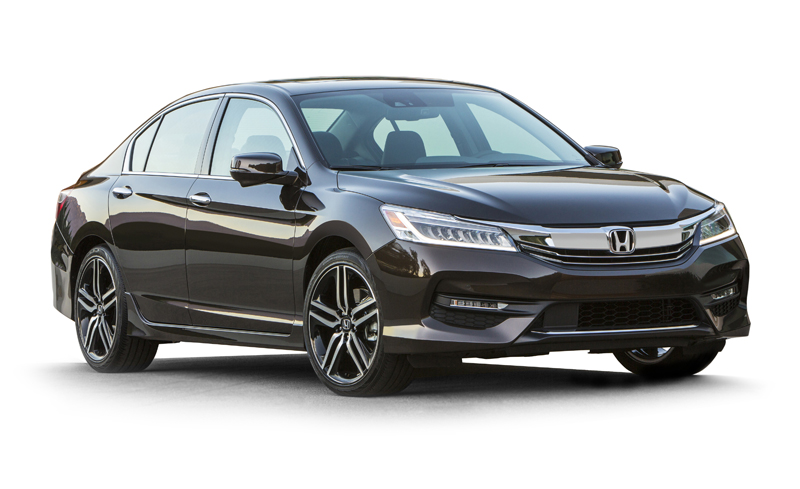
\includegraphics[width=2.7in]{accord.jpg}
\end{figure}

The 2016 Honda Accord sells at many different dealerships in New York City but sell it for more and some for less. We'll assume that the final negotiated price is distributed normally because it's most likely the sum of many different negotiation factors.

Our goal here is to determine the mean price at a certain car dealership in Astoria that people have been saying is \qu{too cheap} and if it's too cheap, Honda corporate may wish to investigate.

\begin{enumerate}



\intermediatesubproblem{Assume that each Accord's price at the Astoria dealership is normal and $\iid$ given the parameters. The nationwide variance for a Honda Accord selling price we're going to assume is $\sigsq = \$1000^2$. You and your colleague go down to the Astoria dealership undercover and ask to buy a Honda. After much negotiation, they will sell it to you for \$19,000 and they will sell it to your colleague for \$18,200 but they sense something suspicious so you hesitate to send another one of your guys down there to do another faux negotiation. Unfortunately, we're going to have to estimate the mean with just $x_1=19000$ and $x_2 = 18200$. What is your best guess of the mean price of Honda Accords sold here? Assume your prior from (a).}\spc{2}

\intermediatesubproblem{Based on this data, we wish to test if this dealership is selling Honda Accords below the manufacturer sugested retail price (MSRP) of \$22,205 --- if so, they would be subject to a fine. Calculate a $p$-value for this test below by using notation from Table~\ref{tab:eqs} but do not solve numerically.}\spc{4}

\hardsubproblem{What is the probability I get a really good deal --- that I can buy a car from these Astoria people for under \$17,000? Use the notation from Table~\ref{tab:eqs} but do not solve numerically.}\spc{3}



\end{enumerate}

\problem This question is about building a model to understand the accuracy of this beverage-filling machine pictured below:

\begin{figure}[htp]
\centering
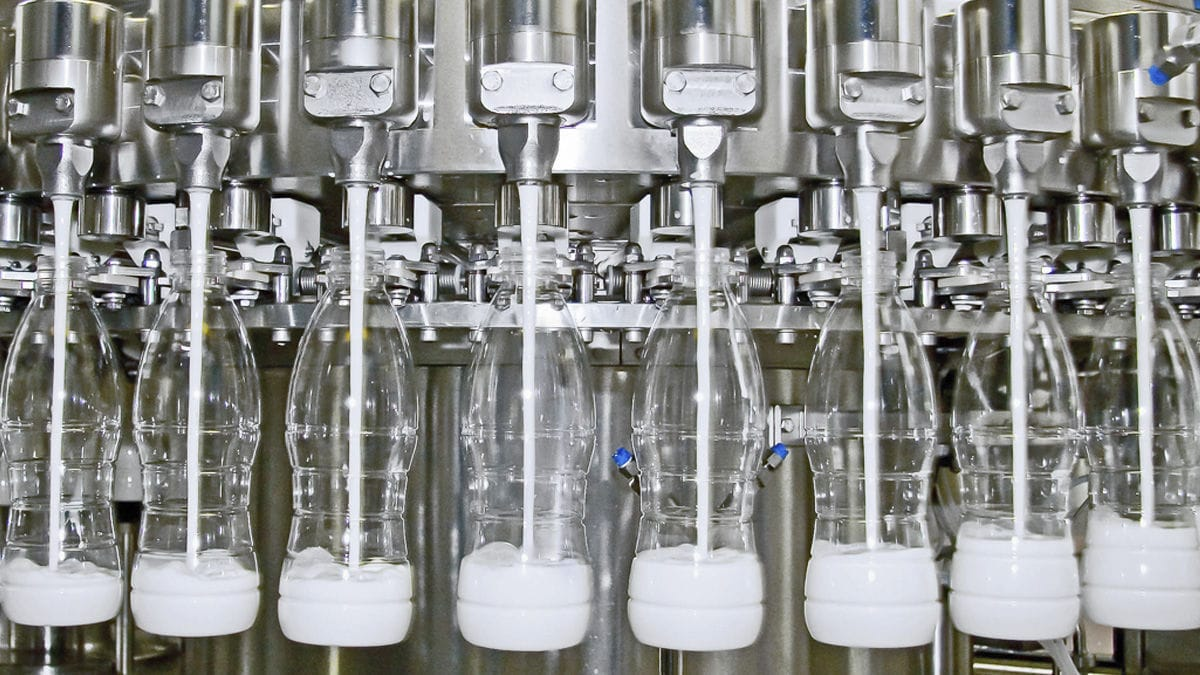
\includegraphics[width=3.7in]{milk_filling.jpg}
\end{figure}

This machine fills 12oz plastic bottles. There is no doubt the mean amount of liquid filled per bottle is 12oz as been determined by the final weights of pallets of filled bottles. But we are uncertain about the variance. We decide to do an experiment and select $n = 21$ bottles at random and measure the amount of liquid in each bottle. Here are the measurements:

\begin{verbatim}
                   12.00 12.05 11.98 11.66 12.05 11.92 12.03
                   12.23 12.36 11.57 12.04 12.10 11.99 12.47
                   12.57 11.83 12.20 12.48 12.14 12.14 12.74
\end{verbatim}

Assume an $\iid$ normal model.

\begin{enumerate}
\easysubproblem{Find the MLE for $\sigsq$.}\spc{1}

\intermediatesubproblem{Under the Jeffrey's prior for $\sigsq$, find the posterior of $\sigsq$ by solving for the parameter values.}\spc{1}

\intermediatesubproblem{Write an expression for the 95\% left-sided credible region for $\sigsq$. This is a one sided CR which will give the upper bound for the machine's variance.}\spc{1}


\intermediatesubproblem{The bottles are actually 13.5oz. This means that you wish to test if $\sigsq > 0.352$ for if so, about 1/100,000 of the bottles will be overfull and that's the tolerance of the factory. Write an expression for the Bayesian p-value of this test.}\spc{2}


\intermediatesubproblem{Write an expression for the probability the next bottle has more than 13oz of liquid.}\spc{2}

%\intermediatesubproblem{Write an expression for the 95\% posterior predictive interval (PI) for the amount of liquid in the next bottle.}\spc{3}
\end{enumerate}


\problem{Now we will move to the Bayesian normal-normal model for estimating both the mean and variance and demonstrate similarities with the classical results.}

\begin{enumerate}

\easysubproblem{If $\Xoneton~|~\theta, \sigsq \iid \normnot{\theta}{\sigsq}$ and $X$ represents all $\Xoneton$. Find the kernel of the posterior if $f(\theta,~\sigsq) \propto \oneover{\sigsq}$. Use the substitution that we made in class $\sum_{i=1}^n (x_i - \theta)^2 = (n-1)s^2 + n(\xbar - \theta)^2$ where $s^2 := \oneover{n-1} \sum_{i=1}^n (x_i -\xbar)^2$. }\spc{8}


\easysubproblem{Using Bayes Rule, break up the posterior into two pieces as we did in class. How are those two pieces distributed?}\spc{2}

\hardsubproblem{Using Bayes Rule, partition the posterior into two differently than the previous question. How are those two pieces distributed?}\spc{2}

\intermediatesubproblem{Using your answer from (b), explain in English how you can create $S$ samples from the posterior distribution that look like $\braces{\bracks{\theta_1, \sigsq_1}, \bracks{\theta_2, \sigsq_2}, \ldots, \bracks{\theta_S, \sigsq_S}}$.}\spc{8}

\hardsubproblem{Using these samples, how would you estimate $\cexpe{\theta}{X}$ and $\cexpe{\sigsq}{X}$?}\spc{5}


\hardsubproblem{Using these samples, how would you estimate a 95\% CR for $\theta$?}\spc{6}

\hardsubproblem{Using these samples, how would you obtain a $p$-val for testing if $\sigsq > 1.364$?}\spc{6}

\hardsubproblem{[MA] Using these samples, how would you estimate $\corr{\theta~|~X}{~\sigsq~|~X}$ i.e. the correlation between the posterior distributions of the two parameters?}\spc{7}

%\easysubproblem{If $\Xoneton~|~\theta, \sigsq \iid \normnot{\theta}{\sigsq}$ and $\theta \sim \normnot{\mu_0}{\tausq}$ write the distribution of $\theta~|~X,\sigsq$. Hint: it's in the notes and it was HW6 6(d). Note this problem is independent of the other problems.}\spc{5}

%\easysubproblem{Find $\cprob{\theta}{X,~\sigsq}$ by using the full posterior kernel from (a) and then conditioning on $\sigsq$. You should get the same answer as we did before the midterm.}\spc{3}

%\easysubproblem{Find $\cprob{\sigsq}{X,~\theta}$ by using the full posterior kernel from (a)  and then conditioning on $\theta$. You should get the same answer as we did before the midterm.}\spc{4}

%\intermediatesubproblem{Show that $\cprob{\sigsq}{X}$ is an inverse gamma distribution and find its parameters.}\spc{4}

%\hardsubproblem{Show that $\cprob{\theta}{X}$ is a non-standard $T$ distribution and find its parameters. Assume the prior $\prob{\theta,~\sigsq} \propto \oneover{\sigsq}$. The answer is in the notes, but try to do it yourself.}\spc{15}


%\hardsubproblem{Show that $\cprob{\sigsq}{X}$ is an inverse gamma and find its parameters. Assume the prior $\prob{\theta,~\sigsq} \propto \oneover{\sigsq}$. The answer is in the notes, but try to do it yourself.}\spc{12}


%\intermediatesubproblem{How does this compare to 2(j)? Note that $X \sim \invgammanot{\alpha}{\beta}$ then $cX \sim \invgammanot{\alpha}{\frac{\beta}{c}}$.}\spc{2}


%\extracreditsubproblem{Prove what you wrote in the previous question: $\cprob{X^*}{X}$ is the non-standard $T$ distribution and find its parameters.}\spc{0}


\hardsubproblem{Explain how to sample from the posterior predictive distribution of for the next observation.}\spc{9}


\easysubproblem{How is $X^*\,|\,X$ distributed assuming the prior $f(\theta, \sigsq) \propto \oneover{\sigsq}$?}\spc{1}

\intermediatesubproblem{[MA] Now consider the informative conjugate prior of $\theta\,|\,\sigsq \sim \normnot{\mu_0}{\frac{\sigsq}{m}}$ and $\sigsq \sim \invgammanot{\overtwo{n_0}}{\overtwo{n_0 \sigsq_0}}$. Find the posterior and demonstrate it that the normal-inverse gamma is conjugate for the normal likelihood with both mean and variance unknown. This is what I did \emph{not} do in class.}\spc{13}

\end{enumerate}

\problem{We model the returns of S\&P 500 here.}

\begin{enumerate}
\easysubproblem{Below are the 16,428 daily returns (as a percentage) of the S\&P 500 dating back to January 4, 1950 and the code used to generate it. Does the data look normal? Yes/no}\spc{0}

\begin{figure}[h]
\centering
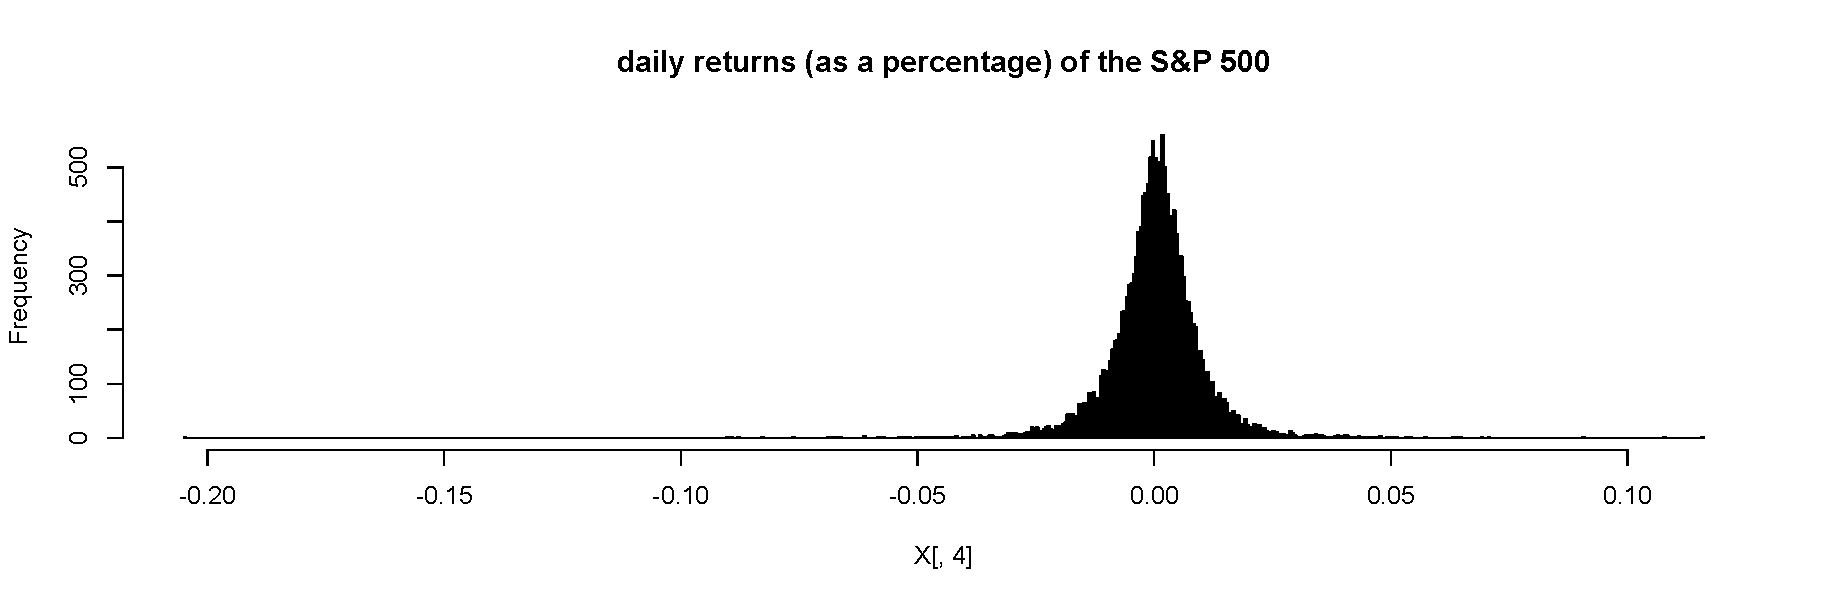
\includegraphics[width=7in]{daily_returns}
\end{figure}

%\begin{verbatim}
%X = read.csv('sp_tot_ret_price_1950.csv')
%n = nrow(X)
%n
%hist(X[,4], br = 1000, 
%  main = 'daily returns (as a percentage) of the S&P 500')
%\end{verbatim}

\intermediatesubproblem{Do you think the data is $\iid$? Explain.}\spc{1}

\intermediatesubproblem{Assume $\iid$ normal data regardless of what you wrote in (a) and (b). The sample average is $\xbar = 0.0003415$ and the sample standard deviation is $s = 0.0096$. Under an objective prior, give a 95\% credible region for the true mean daily return.}\spc{4}

\hardsubproblem{Give a 95\% predictive region for \emph{tomorrow's} return.}\spc{4}

\end{enumerate}

\end{document}


